\documentclass[border=6pt]{standalone}
\usepackage{tikz}
\usepackage[edges]{forest}
\usetikzlibrary{arrows.meta,positioning,calc,decorations.pathreplacing,shapes.geometric}
\begin{document}
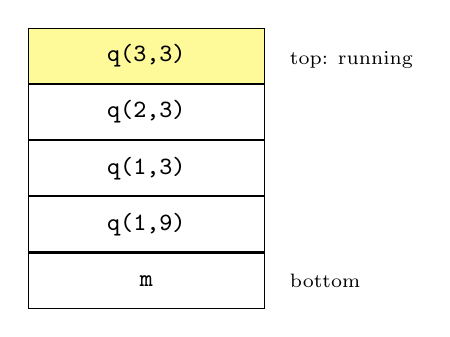
\begin{tikzpicture}[font=\small,rec/.style={draw,minimum width=3.0cm,minimum height=0.7cm,align=center}]
\node[rec] (a) at (0,0) {\texttt{m}};
\node[rec,above=0cm of a] (b) {\texttt{q(1,9)}};
\node[rec,above=0cm of b] (c) {\texttt{q(1,3)}};
\node[rec,above=0cm of c] (d) {\texttt{q(2,3)}};
\node[rec,above=0cm of d,fill=yellow!40] (e) {\texttt{q(3,3)}};
\node[font=\scriptsize,anchor=west] at (1.7,0) {bottom};
\node[font=\scriptsize,anchor=west] at (1.7,2.8) {top: running};
\end{tikzpicture}
\end{document}
